\documentclass[12pt]{extarticle}
\usepackage[protrusion=true]{microtype}
\usepackage[sfdefault]{FiraSans}
\usepackage[T1]{fontenc}
\usepackage[utf8]{inputenc}
\usepackage{adjustbox}
\usepackage{algorithm}
\usepackage{algorithmic}
\usepackage{amsfonts}
\usepackage{amsmath}
\usepackage{amssymb}
\usepackage[style=apa]{biblatex}
\addbibresource{references.bib}
\usepackage{booktabs}
\usepackage{breqn}
\usepackage{enumitem}
\usepackage{float}
\usepackage{geometry}
\usepackage{graphicx}
\usepackage{hyperref}
\usepackage{lipsum}
\usepackage{longtable}
\usepackage{multirow}
\usepackage{pdfpages}
\usepackage{pgfgantt}
\usepackage{setspace}
\usepackage{subcaption}
\usepackage{tabularx}
\usepackage{tikz}
\usepackage{xcolor}

\DeclareLanguageMapping{english}{english-apa}

\geometry{letterpaper, left=1in, right=1in, top=1in, bottom=1in,}

\definecolor{primary}{RGB}{0,120,215}
\definecolor{secondary}{RGB}{255,87,34}
\definecolor{background}{RGB}{245,245,245}
\definecolor{blue}{RGB}{0,62,126}

\pagecolor{background}

\hypersetup{colorlinks=true, linkcolor=primary, filecolor=secondary, urlcolor=primary, citecolor=black}

\AtBeginBibliography{\hypersetup{urlcolor=black}}

\setstretch{1.15}

\setlength{\bibhang}{0.5in}

\setlength\bibitemsep{1.5\itemsep}

\setlength{\parindent}{0pt}

\nocite{*}

\begin{document}

\newcommand{\mytitlepage}[2]{
    \thispagestyle{empty}
    \begin{tikzpicture}[remember picture, overlay]
        \node [inner sep=0pt] at (current page.center) {#1};
        \node [ anchor=center, inner sep=1.25cm, rectangle, fill=blue!70!white, fill opacity=0, text opacity=1, minimum height=0.2\paperheight, minimum width=\paperwidth, text width=0.8\paperwidth, font=\fontfamily{pnc}\selectfont ] at (current page.center) {#2};
        \node [anchor=south east, outer sep=3pt] at (current page.south east) {
\includegraphics[width=0.33\paperwidth]{images/logo.png}};
    \end{tikzpicture}
    \newpage
}

\mytitlepage{\includegraphics[width=\paperwidth]{images/background.png}} {
    \centering
    \fontfamily{phv}
    \vspace{-130pt}
    {\Large \bfseries \par}
    \vspace{8pt}
    {\Huge \bfseries Advanced Generative Chatbot Design \par}
    \vspace{24pt}
    {
        \begin{center}
            \begin{tabular*}{\textwidth}{@{\extracolsep{\fill}}ccc}
                \LARGE Eric Barnes & \LARGE Massimiliano Repupilli & \LARGE Jonathan Agustin \\
            \end{tabular*}
        \end{center}
    }
}

\pagenumbering{arabic}

\begin{abstract}

\noindent This study explores the creation of open source conversational chatbots, capitalizing on transformer networks and the nuanced application of transfer learning from pretrained models. We unpack the methods, experimental processes, outcomes, and nuanced analyses involved in fine-tuning BERT, DistilBERT, and RoBERTa with version 2 of the Stanford Question Answering Dataset (SQuAD). We find that RoBERTa outperforms its counterparts, which highlights the importance of optimized pretraining procedures. Overall, all three models were consistently challenged when handling unanswerable questions, indicating an area for future exploration.

\end{abstract}

\section{Introduction}

AI constantly faces the challenge of creating chatbots that can effectively mimic human interaction across various topics. Despite advances in deep learning, understanding language and managing dialogues remain complex. Our project focuses on developing an engaging chatbot for a wide range of subjects, using Open Source NLP techniques. We leverage transfer learning from pretrained models like BERT. This exploration chronicles our process, including literature review, data collection, model design, training methods, evaluation, and analysis. We compare different three transformer models and report statistics. Ultimately, we aim to contribute to future research in conversational AI systems.

\section{Related Work}

BERT \textcite{devlin2018bert} advances NLP through introducing a way to learn from before and after a position within a text, which was not done previously. This bidirectional approach enhanced BERT's adaptability, making it a top solution for many tasks with minimal adjustment. Subsequent studies concentrate on optimizing BERT's pretraining methods. RoBERTa emphasized the importance of parameters like batch size, training duration, and dataset size. DistilBERT streamlined the essence of BERT, achieving a compact model without compromising on performance, bridging the gap between computational efficiency and effectiveness.

\section{Exploration}

\subsection{SQuAD}

The Stanford Question Answering Dataset (SQuAD) is a popular dataset for training Q\&A models. We use the second version of SQuAD, which improves upon its previous version through adding unanswerable questions. This impossibility challenges a model's ability to understand and interpret text.  We aim to advance these transformer technologies through leveraging existing pretrained models, datasets, and distillations.

SQuAD 2.0 challenges a model's ability to understand and interpret text.

\begin{table}[h!]
    \centering
    \caption{Overview of the SQuADv2 Dataset}
    \begin{tabular}{@{}ll@{}}
        \toprule
            \textbf{Detail}          & \textbf{Information or Statistics} \\
        \midrule
            Dataset Name & squad\_v2 \\
            Description & Combines 100,000 questions with over 50,000 unanswerable questions \\
                                    & written adversarially by crowdworkers to look similar to answerable ones. \\
                                    & Systems must determine when no answer is supported by the paragraph \\
                                    & and abstain from answering. \\
            Citation                & \textit{Rajpurkar, Pranav et al. SQuAD: 100,000+ Questions for Machine} \\
                                    & \textit{Comprehension of Text, arXiv e-prints, 2016.} \\
            Homepage                & \href{https://rajpurkar.github.io/SQuAD-explorer/}{SQuAD Explorer} \\
        \midrule
            Train Examples          & 130,319 \\
            Validation Examples     & 11,873 \\
        \bottomrule
    \end{tabular}
    \label{tab:my-table}
\end{table}

Table 1 provides details about the SQuAD 2.0 dataset. Unanswerable questions tests not only information retrieval skills but also discernment in recognizing when text does not contain an answer.

\begin{figure}[h!]
    \centering
    \begin{adjustbox}{center, scale=0.8}
    \begin{tikzpicture}[font=\sffamily, every matrix/.style={ampersand replacement=\&,column sep=2cm,row sep=2cm}, source/.style={draw,thick,rounded corners,fill=yellow!20,inner sep=.3cm}, process/.style={draw,thick,circle,fill=blue!20}, sink/.style={source,fill=green!20}, datastore/.style={draw,very thick,shape=datastore,inner sep=.3cm}, dots/.style={gray,scale=2}, to/.style={->,>=stealth',shorten >=1pt,semithick,font=\sffamily\footnotesize}]
    \matrix{
        \node[source] (question) {Question: When were the Normans in Normandy?}; \& \\
        \node[process] (answers) {Answers}; \& \\
        \node[sink] (context) {Context: The Normans (Norman: Nourmands; French: Normands; Latin: Normanni) were the people...}; \& \\
    };
    \draw[to] (question) -- (answers);
    \draw[to] (answers) -- (context);
    \draw[to,shorten <=1pt] (context) -- ++(0,1) -| (question) node[near start,above] {supports};
    \end{tikzpicture}
    \end{adjustbox}
    \caption{Diagram representing the relationship between question, answer, and context.}
    \label{fig:qac_diagram}
\end{figure}

Figure 1 shows the steps involved in answering a question. The model is limited to only the context when answering a question.

\subsection{BERT}

BERT (Bidirectional Encoder Representations from Transformers) significantly advanced the field of natural language understanding with its innovative approach to contextual encoding. This model, introduced by \textcite{devlin2018bert}, allows for highly effective transfer learning, particularly in the realm of language comprehension tasks. We explore the innovative bidirectional nature of this model and measure its effectiveness.

\subsection{DistilBERT}
\textcite{sanh2019distilbert} introduced DistilBERT, a distilled version of the original BERT model that retains most of its performance characteristics with significantly fewer resources. Our implementation involved fine-tuning and exploring its efficient architecture, which is ideal for resource-restricted environments.

\subsection{RoBERTa}
RoBERTa, \textcite{liu2019roberta}, refines pre-training process through, for example, modifying the masking pattern applied to training data and through extending the training period. Our implementation of RoBERTa explored its versatility in generating contextually appropriate multilingual responses.


\section{Model Development}

Our strategy leveraged the HuggingFace Model Hub and other third-party libraries. Three pretrained models---BERT, DistilBERT, and RoBERTa---were inputted into an encoder-decoder pipline. Initialization with pretrained weights was important as it allowed models to capitalize on previously acquired training activitys. The models were trained using A100 and T4 GPUs on Google Colab. This cloud setup enabled remote development at little to no cost. Persistence between sessions was achieved through Google Drive, which allowed us to save and load checkpoints.

\section{Training}

Handling comprehensive datasets like SQuAD in NLP tasks require preprocessing, including tokenizing sentences, adjusting sequence lengths, and calculating indices. The process is often time-consuming and susceptible to errors. We streamlined training with using a third-party library called \texttt{txtai} (see code in the Appendix). At the beginning, we manual preprocessed the datasets, but it was difficult. Importing the library allowed for more concise code and allowed us to go to the next step without ad-hoc trial-and-error data manipulation.

\section{Evaluation}

After training a model, we used the \texttt{evaluate} library from HuggingFace's Transformer library. We used the official SQuADv2 to measure model predictions. The results were outputted, saved, and published. Despite the need to handle unanswerable questions, the evaluation phase provided crucial insight in improving overall performance.

\section{Results}

RoBERTa outperformed its counterparts, which highlights the importance of optimized pretraining procedures. Models were consistently challenged when handling unanswerable questions, indicating an area for future exploration.

\begin{itemize}
    \item GitHub
    \begin{itemize}
        \item[] \href{https://github.com/aai520-group6/project}{https://github.com/aai520-group6/project}
    \end{itemize}
    \item BERT
    \begin{itemize}
        \item[] \href{https://huggingface.co/aai520-group6/bert-finetuned-uncased-squad_v2}{https://huggingface.co/aai520-group6/bert-finetuned-uncased-squad\_v2}
    \end{itemize}
    \item DistilBERT
    \begin{itemize}
        \item[] \href{https://huggingface.co/aai520-group6/distilbert-finetuned-uncased-squad_v2}{https://huggingface.co/aai520-group6/distilbert-finetuned-uncased-squad\_v2}
    \end{itemize}
    \item RoBERTa
    \begin{itemize}
        \item[] \href{https://huggingface.co/aai520-group6/roberta-finetuned-uncased-squad_v2}{https://huggingface.co/aai520-group6/roberta-finetuned-uncased-squad\_v2}
    \end{itemize}
\end{itemize}

\begin{figure}[h!]
    \centering
    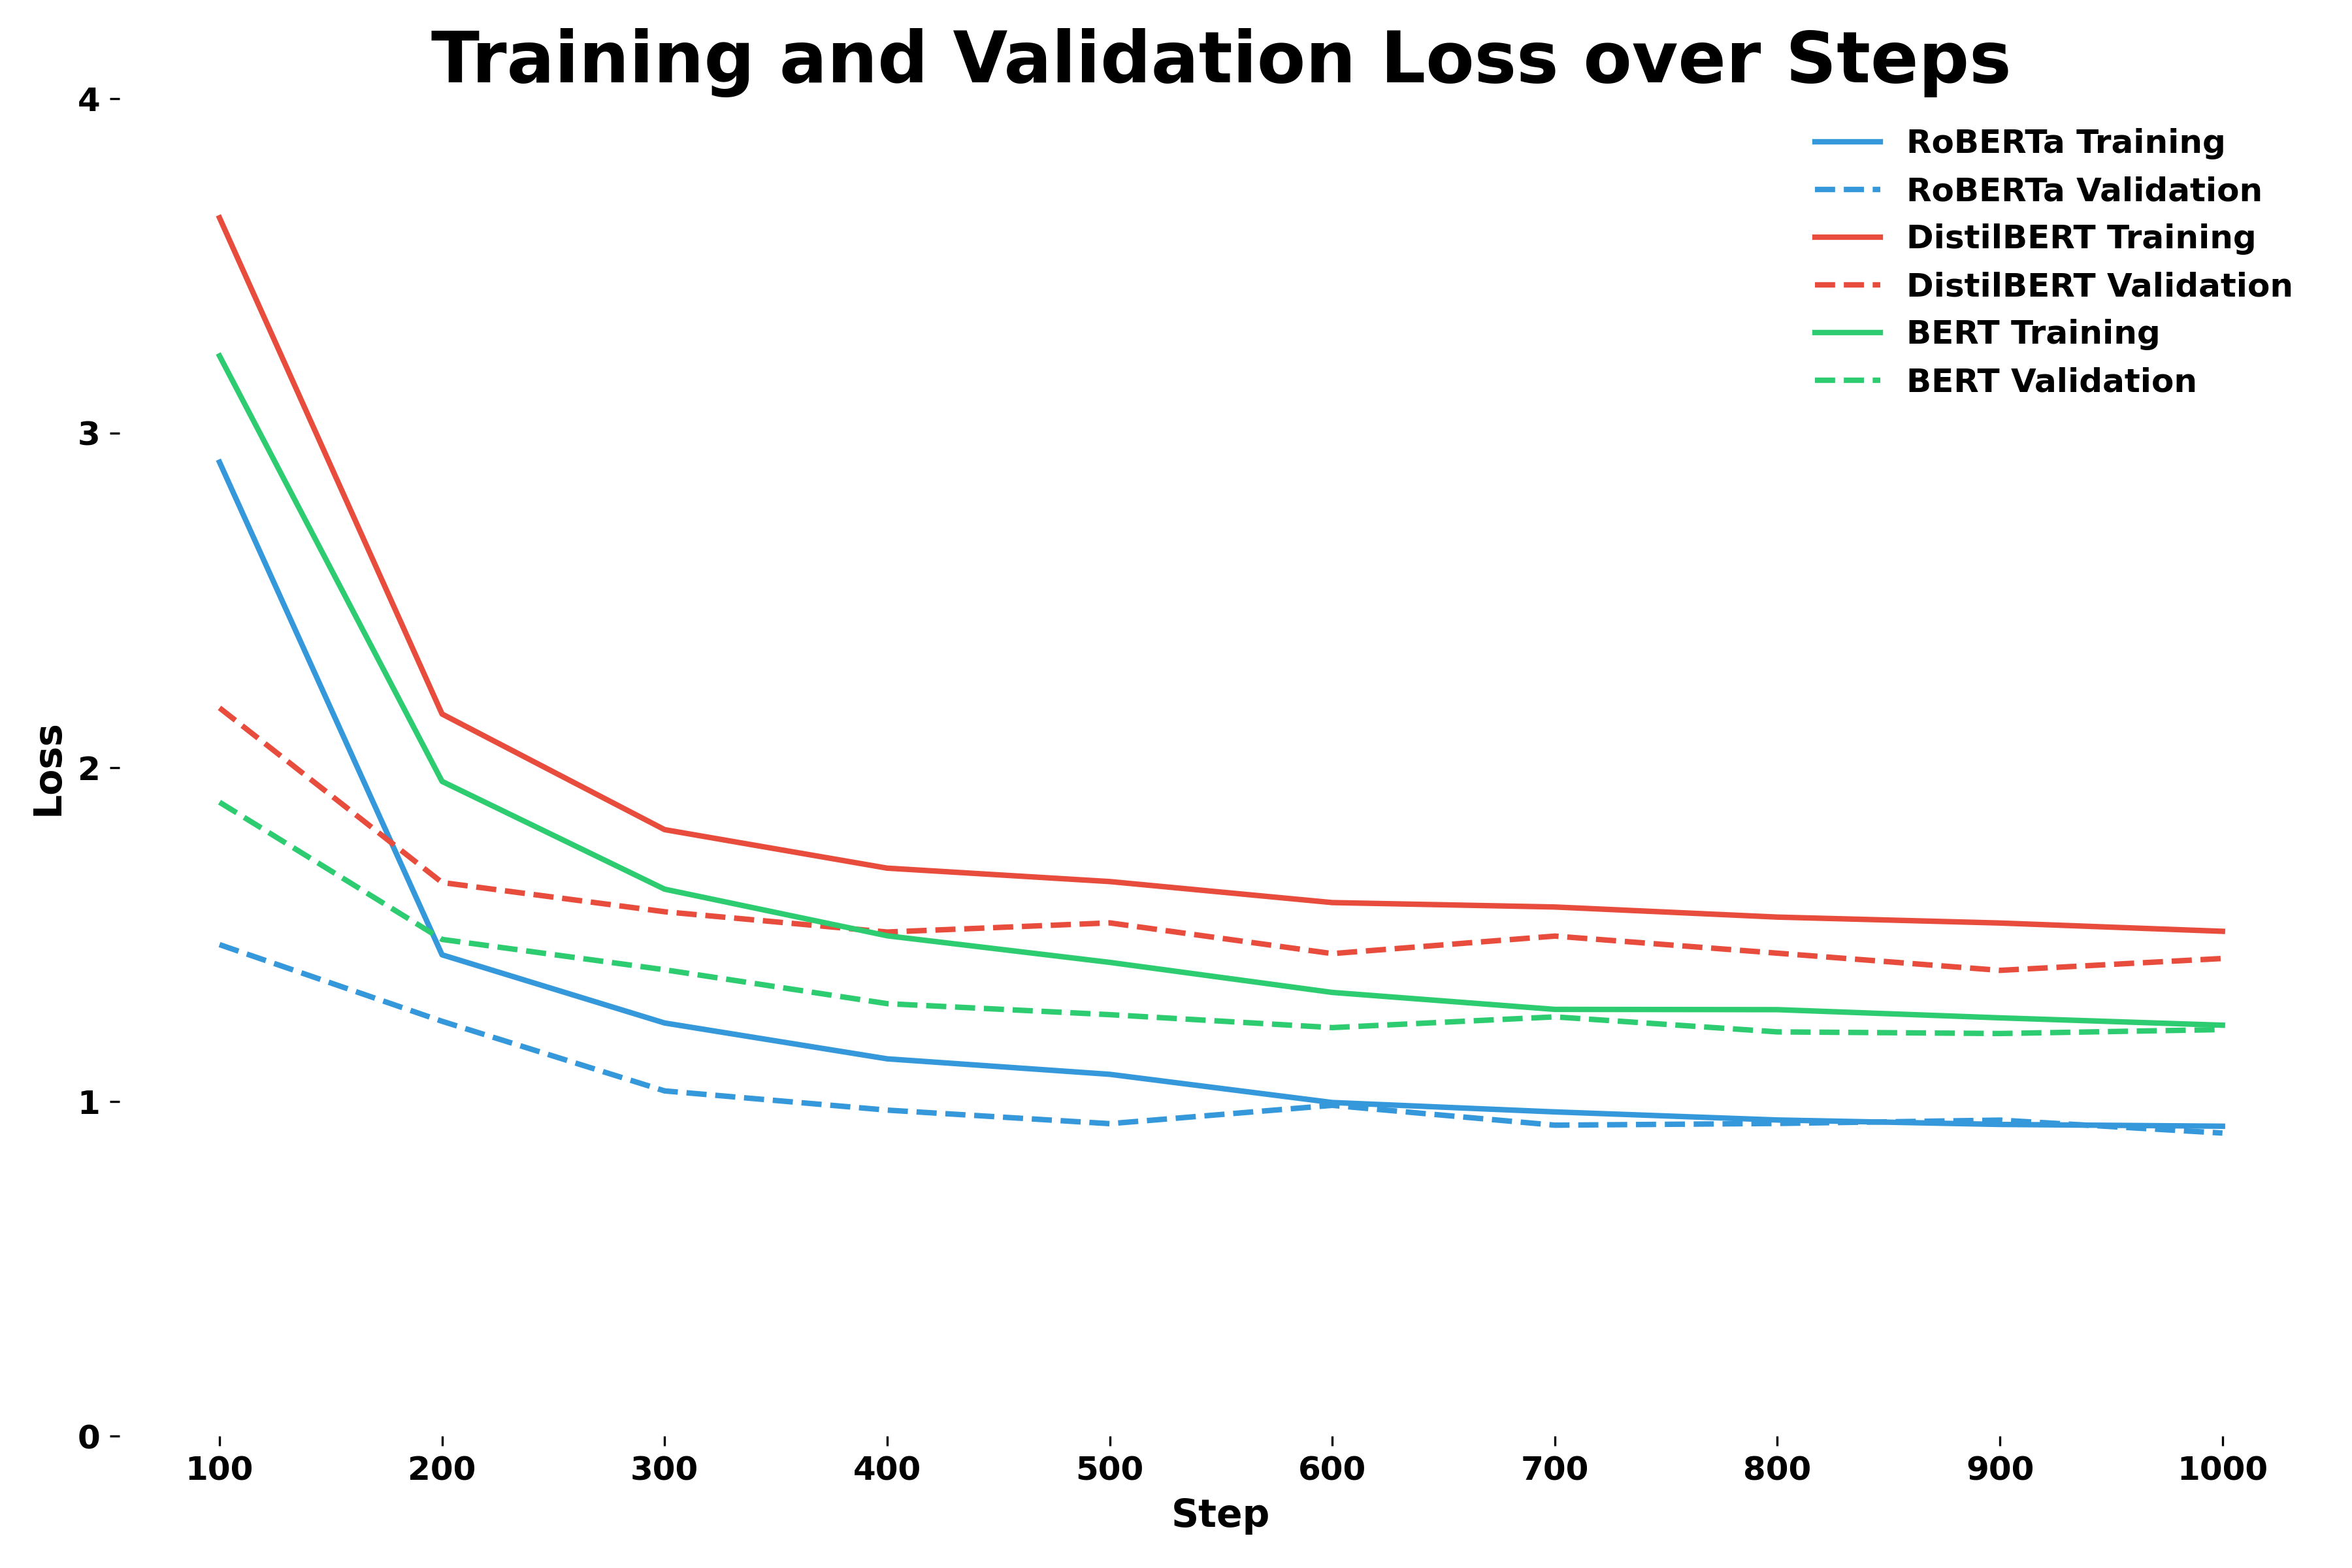
\includegraphics[width=0.8\textwidth]{images/loss-over-time.png}
    \caption{Visualization of model loss over time during training.}
    \label{fig:loss}
    \end{figure}

\begin{figure}[h]
    \centering
    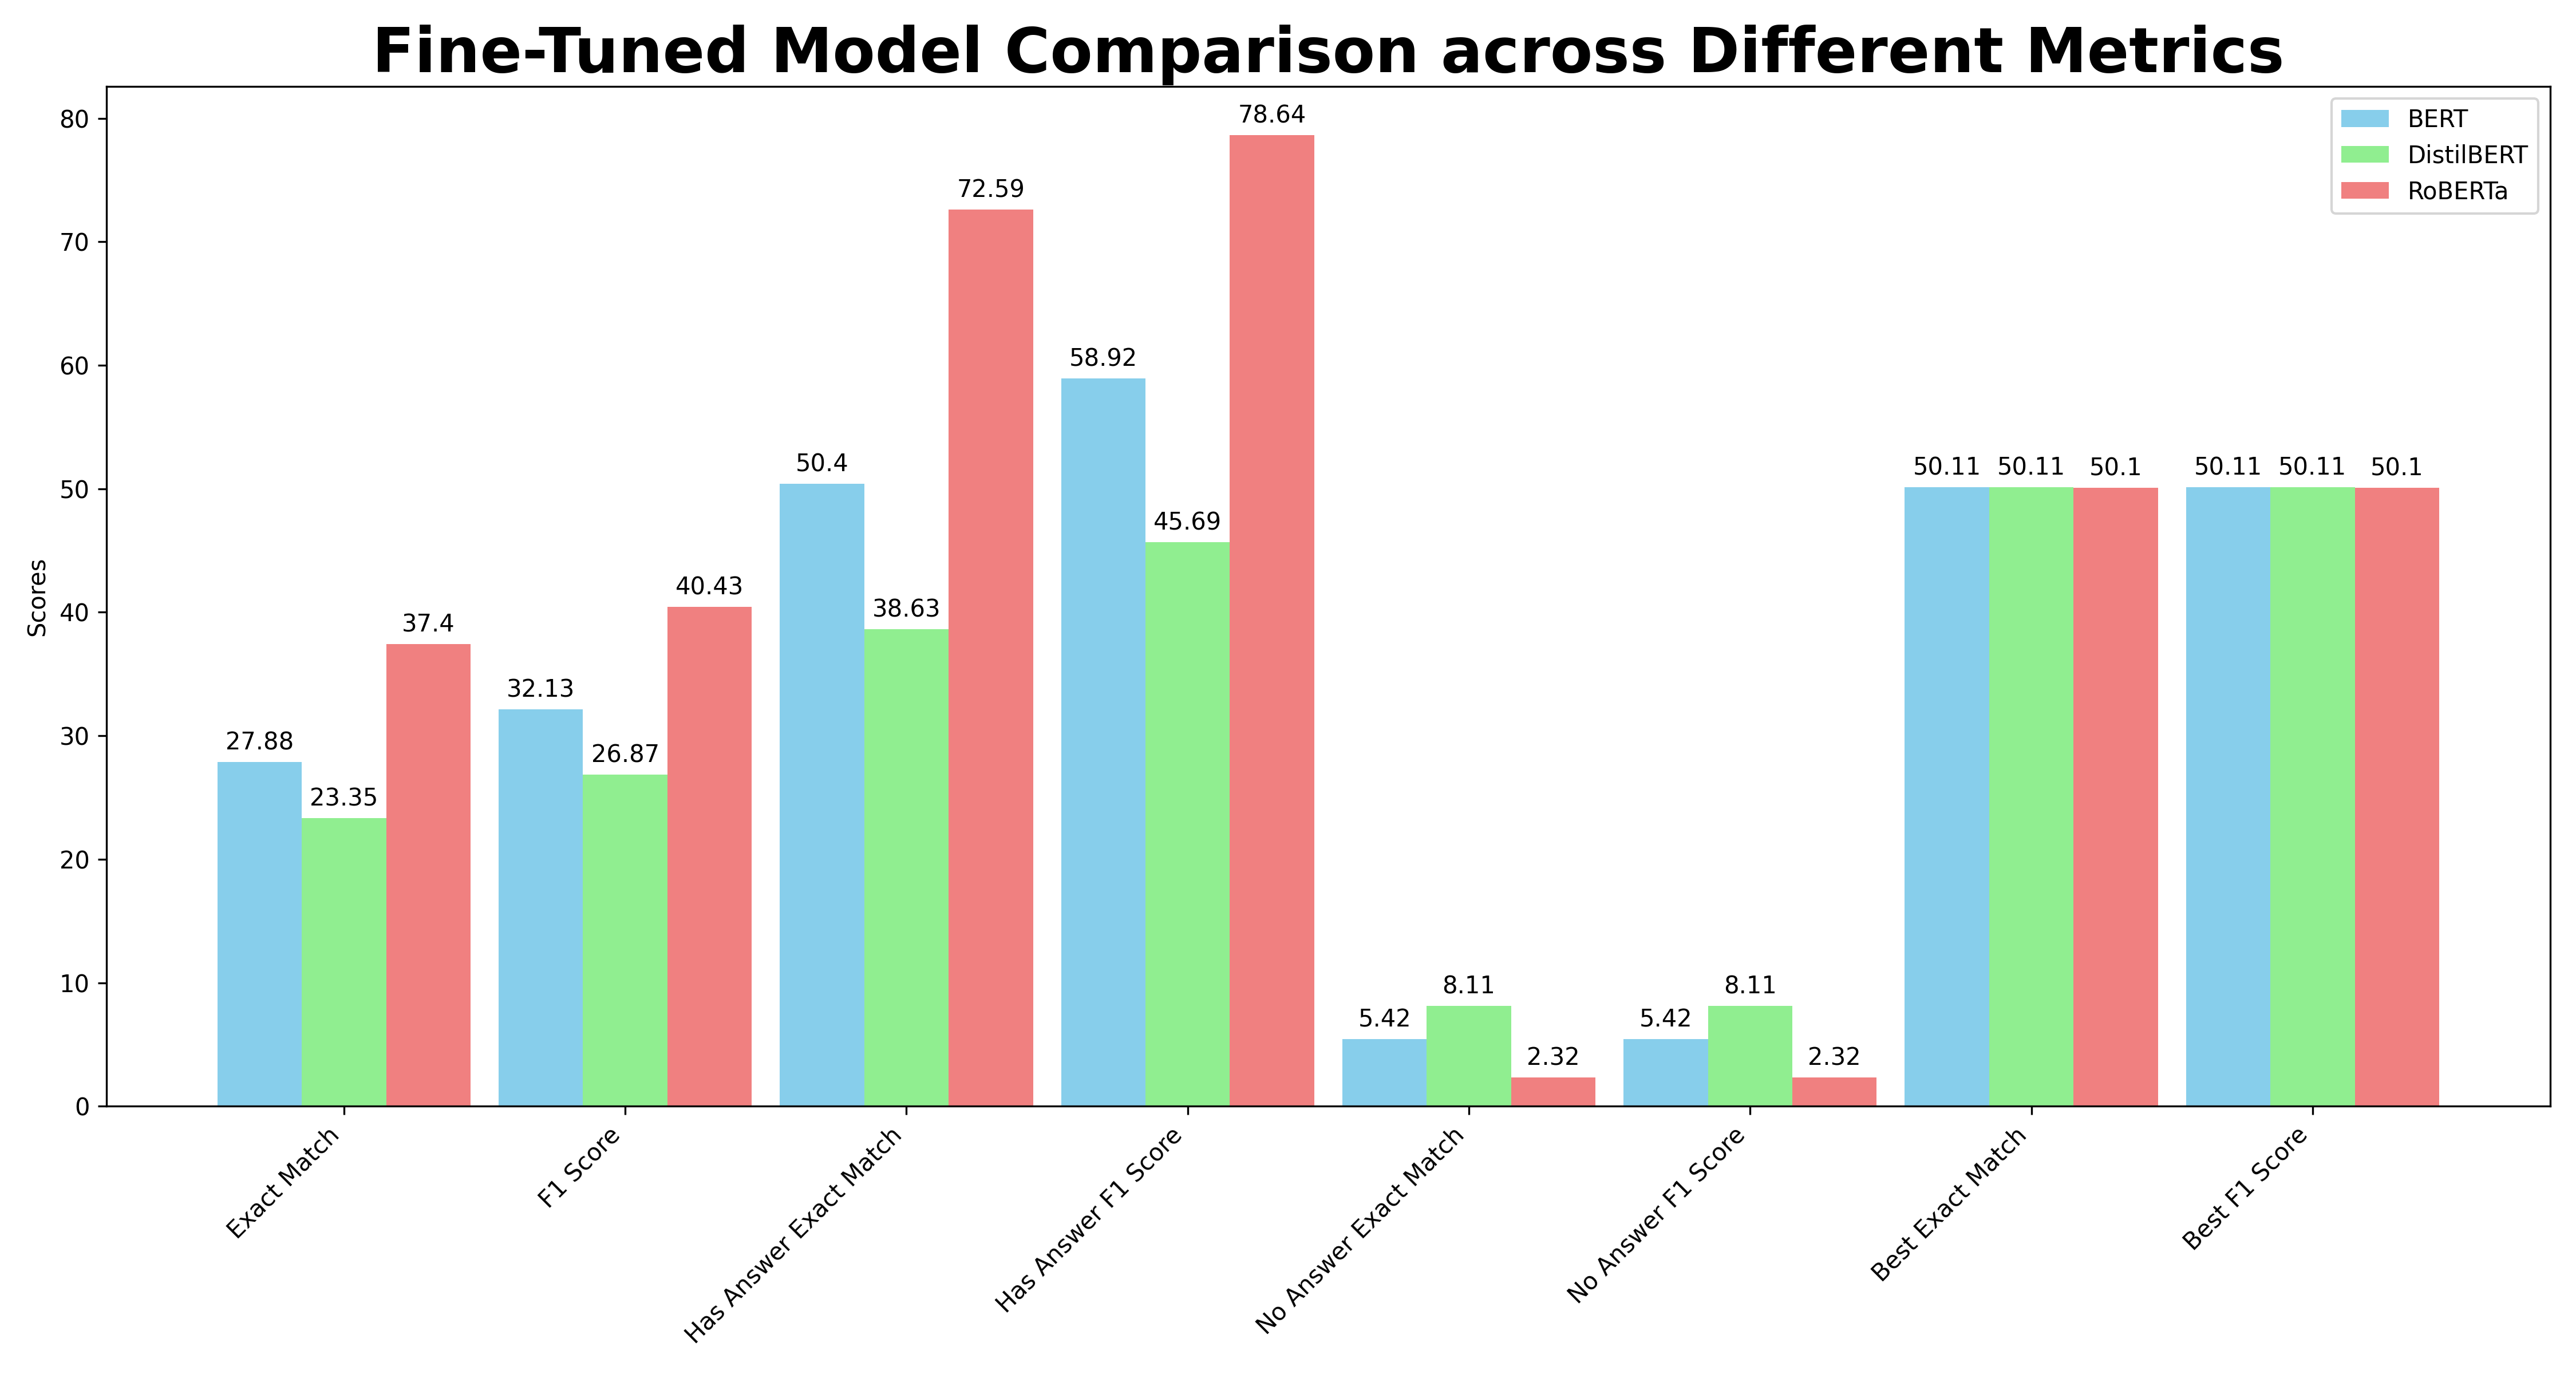
\includegraphics[width=0.8\textwidth]{images/model-metric-comparison.png}
    \caption{Comparison of fine-tuned models on various metrics.}
    \label{fig:comparison}
    \end{figure}

\begin{center}
    \begin{tabular}{|l|c|c|c|}
    \hline
    \multicolumn{4}{|c|}{\textbf{Fine-tuned Model Comparison}} \\
    \hline
    Metric & BERT & DistilBERT & RoBERTa \\
    \hline
    Total Examples & 11,873 & 11,873 & 11,873 \\
    \hline
    Exact Match & 27.878 & 23.347 & 37.404 \\
    F1 Score & 32.130 & 26.870 & 40.428 \\
    \hline
    Total with Answer & 5,928 & 5,928 & 5,928 \\
    Has Answer Exact Match & 50.405 & 38.630 & 72.588 \\
    Has Answer F1 Score & 58.920 & 45.686 & 78.644 \\
    \hline
    Total without Answer & 5,945 & 5,945 & 5,945 \\
    No Answer Exact Match & 5.416 & 8.108 & 2.321 \\
    No Answer F1 Score & 5.416 & 8.108 & 2.321 \\
    \hline
    Best Exact Match & 50.114 & 50.114 & 50.097 \\
    Best F1 Score & 50.114 & 50.114 & 50.097 \\
    \hline
    \end{tabular}
\end{center}

\section{Discussion}

Our exploration shows the relative ease of transfer learning in dialog-oriented tasks. RoBERTa's superior performance shows the importance of nuanced training and specific selections of hyperparameters like dataset size and training duration. The models were able to answer questions with high accuracy, but struggled with unanswerable questions. Future iterations should emphasize training with unanswerable questions to enhance a model's discernment abilities. Solving these issues will allow for conversational agents to rise to the level of for real-world human interaction.

\subsection{Challenges and Limitations}

We faced Out-of-Memory (OOM) issues using Google Colab. These issues often required us to adjust our approach, such as using smaller data batches or simplifying model structures. Despite its advanced features, Colab sometimes had performance limitations, and session management was disruptive, causing delays in our workflow. The interactive terminal in Colab was often slow, especially through a VPN. The speed was good enough for notebooks and we often used the notebook to invoke terminal commands. This slowed down testing and debugging, but we were able to work around this limitation.

\section{Conclusion}

We explored conversational chatbots, fine-tuning transformer networks to enhance a multi-turn dialog capability. Our exploration and analysis is all published to open source, guiding future endeavors towards refining conversational AI technologies.

\newpage

\printbibliography

\newpage

\appendix
\section{Appendix}

\subsection{Training Hyperparameters}
\begin{table}[h]
\centering
\begin{tabular}{|l|l|}
\hline
\textbf{Hyperparameter}              & \textbf{Value} \\ \hline
Learning Rate                        & 2e-05          \\ \hline
Train Batch Size                     & 64             \\ \hline
Eval Batch Size                      & 64             \\ \hline
Gradient Accumulation Steps          & 4              \\ \hline
Total Train Batch Size (effective)   & 256            \\ \hline
Optimizer                            & Adam           \\ \hline
Optimizer Betas                      & (0.9, 0.999)   \\ \hline
Optimizer Epsilon                    & 1e-08          \\ \hline
Learning Rate Scheduler Type         & Linear         \\ \hline
\end{tabular}
\caption{Configured Training Hyperparameters for Model Development}
\label{tab:hyperparameters}
\end{table}


\end{document}
